\documentclass[conference]{IEEEtran}

\usepackage[spanish]{babel}
\usepackage[utf8]{inputenc}
\usepackage{graphicx}
\usepackage{amsmath}
\usepackage{siunitx}
\usepackage{float}
\usepackage{booktabs}
\usepackage{cite}
\usepackage{listings}
\usepackage{xcolor}
\usepackage{hyperref}

\hypersetup{
    colorlinks=true,
    linkcolor=black,
    citecolor=black,
    urlcolor=blue
}

\lstdefinestyle{mystyle}{
    backgroundcolor=\color{white},
    commentstyle=\color{green!50!black},
    keywordstyle=\color{blue},
    numberstyle=\tiny\color{gray},
    stringstyle=\color{red},
    basicstyle=\ttfamily\footnotesize,
    breaklines=true,
    captionpos=b,
    numbers=left,
    numbersep=5pt
}

\usepackage{fancyhdr}
\usepackage{graphicx}

% ------------------------------------------------------------------
% ENCABEZADO INSTITUCIONAL (logo + programa + periodo)
% IMPORTANTE: debes subir el archivo "LogoUMNG.png" (escudo de la
% Universidad Militar Nueva Granada) a la raiz de este proyecto en
% Overleaf para que el encabezado se muestre correctamente.
% ------------------------------------------------------------------
\newcommand{\MYhead}{\smash{\scriptsize
\hfil\parbox[t][\height][t]{\textwidth}{\centering
\begin{picture}(0,0)
\put(-0,-12){\includegraphics[width=16mm]{LogoUMNG.png}}
\end{picture}
\hspace{6.5cm}
ELEMENTOS FINITOS \hspace{6.5cm} Periodo\\
\hspace{6.5cm} PROGRAMA DE INGENIERÍA MECATRÓNICA \hspace{3.8cm} 2026-2\\
\underline{\hspace{\textwidth}}
}}\hfil\hbox{}}

\makeatletter
\def\ps@headings{
\def\@oddhead{\MYhead}
\def\@evenhead{\MYhead}
\def\@oddfoot{\hfil\footnotesize\thepage\hfil}
\def\@evenfoot{\hfil\footnotesize\thepage\hfil}}
\makeatother

\pagestyle{headings}
\setlength{\headheight}{35pt}
\addtolength{\textheight}{-1\baselineskip}
\lstset{style=mystyle}

% ------------------------------------------------------------------
% TÍTULOS DE SECCIÓN MÁS GRANDES Y EN NEGRILLA
% ------------------------------------------------------------------
\makeatletter
\def\section{\@startsection{section}{1}{\z@}{1.5ex plus 1.5ex minus 0.5ex}%
{0.7ex plus 1ex minus 0ex}{\normalfont\large\bfseries\centering\scshape}}%
\def\subsection{\@startsection{subsection}{2}{\z@}{1.5ex plus 1.5ex minus 0.5ex}%
{0.7ex plus .5ex minus 0ex}{\normalfont\normalsize\bfseries}}%
\makeatother

\begin{document}

\title{
PARCIAL ELEMENTOS FINITOS PRIMER CORTE
}

\author{

\and
\IEEEauthorblockN{Nicolas Sebastián Triviño Muñoz}
\IEEEauthorblockA{
7004312\\
est.nicolas.strivino@unimilitar.edu.co
}
\and
\IEEEauthorblockN{Daniel Garcia Araque}
\IEEEauthorblockA{
7004185\\
est.daniel.garciaa@unimilitar.edu.co
}
}

\maketitle
\thispagestyle{headings}

\section*{Resumen}

En el presente informe se desarrolla el Parcial I de la asignatura de Elementos Finitos, el cual está compuesto por cinco problemas que abarcan distintas áreas de aplicación del Método de Elementos Finitos (MEF): análisis estructural axial, análisis estructural a flexión, análisis térmico y análisis magnetostático. En los dos primeros puntos se estudia una barra de hormigón de sección transversal variable —una de sección maciza y otra de sección hueca— sometida a carga axial, resuelta mediante el método de la matriz de rigidez con tres elementos y posteriormente validada mediante simulación en ANSYS, incluyendo el estudio de independencia de malla y el cálculo del error porcentual. En el tercer punto se aborda el análisis de deformación y esfuerzos de una viga de acero de perfil tipo ``I'' sometida a una carga de 50 toneladas, empleando el método de elementos finitos en dos dimensiones a través de la herramienta PDE Tool de MATLAB. El cuarto punto corresponde a la simulación térmica estática, en tres dimensiones y mediante ANSYS, de un caldo de costilla con dos papas al interior de una olla de aluminio de 5 litros, evaluando la distribución de temperatura del sistema. Finalmente, en el quinto punto se realiza una simulación magnetostática en tres dimensiones de un par de bobinas de Helmholtz empleadas para la estimulación muscular del antebrazo, analizando el comportamiento del campo magnético generado. En conjunto, estos cinco problemas permiten evidenciar la versatilidad del MEF como herramienta numérica aplicable tanto a problemas estructurales clásicos como a fenómenos térmicos y electromagnéticos de interés en la ingeniería mecatrónica.

\section{Introducción}

El Método de los Elementos Finitos (MEF) es una técnica numérica que permite aproximar la solución de ecuaciones diferenciales que gobiernan el comportamiento físico de sistemas continuos, mediante la discretización del dominio en elementos más simples conectados por nodos \cite{zienkiewicz2013}\cite{bathe1996}. Su versatilidad permite abordar, bajo un mismo marco matemático, problemas de naturaleza estructural, térmica y electromagnética.

En este parcial se desarrollan cinco problemas: dos barras de hormigón de sección variable (maciza y hueca) sometidas a carga axial, resueltas mediante el método de la matriz de rigidez y validadas en ANSYS; una viga de acero de perfil ``I'' analizada a flexión mediante MATLAB PDE Tool; la simulación térmica en régimen estacionario de una olla con caldo de costilla en ANSYS; y la simulación magnetostática de un par de bobinas de Helmholtz. El planteamiento, desarrollo y análisis de resultados de cada uno se presenta en su sección correspondiente.

\section{Marco Teórico}

El MEF consiste en dividir un dominio continuo en un número finito de elementos interconectados por nodos, sobre los cuales se plantean funciones de interpolación que aproximan el campo de la variable de interés (desplazamiento, temperatura o potencial magnético, según el caso) \cite{logan2012}\cite{reddy2005}.

En problemas estructurales axiales, como los de los puntos 1 y 2, cada elemento se representa mediante una matriz de rigidez local que relaciona las fuerzas nodales con los desplazamientos, en función del área transversal, el módulo de elasticidad y la longitud del elemento; el ensamble de estas matrices locales conduce a la matriz de rigidez global del sistema, la cual, tras aplicar las condiciones de frontera, permite obtener el vector de desplazamientos nodales \cite{logan2012}.

En problemas de esfuerzo plano bidimensional, como el del punto 3, el dominio se discretiza en elementos triangulares de deformación constante (CST, \textit{Constant Strain Triangle\/}), donde cada nodo posee dos grados de libertad ($u_x$, $u_y$); la matriz de deformación-desplazamiento $B$ relaciona estos desplazamientos nodales con las deformaciones dentro del elemento, y junto con la matriz constitutiva $D$ permite obtener la matriz de rigidez elemental y, posteriormente, los esfuerzos mediante $\sigma=D\varepsilon$ \cite{reddy2005}.

En el análisis térmico estacionario (punto 4), el MEF resuelve la ecuación de conducción de calor de Fourier, en la cual el flujo de calor depende del gradiente de temperatura y de la conductividad térmica de cada material presente en el dominio; la formulación resulta análoga a la del problema estructural, sustituyendo la rigidez mecánica por la conductancia térmica de cada elemento \cite{incropera2011}.

Por último, en el análisis magnetostático (punto 5), el MEF resuelve las ecuaciones de Maxwell en su forma estacionaria, particularmente la ley de Ampère, para determinar la distribución del campo magnético generado por las bobinas de Helmholtz; en este caso, el potencial magnético vectorial cumple un rol análogo al del desplazamiento o la temperatura en los problemas anteriores \cite{sadiku2018}.

%======================================================================
% A partir de aquí se desarrollan los cinco puntos del parcial.
% Cada sección contiene la estructura sugerida (a, b, c) según el
% enunciado; complementar con el desarrollo matemático, las capturas
% de ANSYS/MATLAB y el análisis de resultados correspondiente.
%======================================================================

\section{Punto 1 -- Barra de hormigón de sección maciza}

Los puntos 1 y 2 abordan el análisis de una barra de hormigón de 2.80 m de longitud, cuya sección transversal rectangular varía linealmente a lo largo de su eje. En este primer punto se trabaja con la barra de \textbf{sección maciza}: varía desde 60$\times$80 cm en el empotramiento hasta 30$\times$50 cm en el extremo libre, donde se aplica una carga axial de tracción $P=80$ ton (Fig.~\ref{fig:p1_datos}). La barra se discretiza en tres elementos de sección uniforme —cuya área equivale a la sección transversal real evaluada en el punto medio de cada tramo—, se obtiene la solución analítica mediante el método de la matriz de rigidez, y se contrasta con una simulación en ANSYS, reportando la curva de independencia de malla, las figuras de deformación, esfuerzo de Von Mises y factor de seguridad, y el error entre ambos resultados.

\begin{figure}[H]
\centering
\includegraphics[width=0.48\textwidth]{barra_datos_punto1.png}
\caption{Barra de hormigón -- geometría y datos del Punto 1}
\label{fig:p1_datos}
\end{figure}

\subsection{1A. Modelado por matriz de rigidez}

\subsubsection*{Datos}
\begin{itemize}
    \item Base inicial: $b_o = 0.30$ m
    \item Base final: $b_L = 0.60$ m
    \item Altura inicial: $h_o = 0.50$ m
    \item Altura final: $h_L = 0.80$ m
    \item Longitud de la barra: $L = 2.80$ m
    \item Carga aplicada: $P = 80$ ton
    \item Módulo de elasticidad: $E = 2.2\times10^{6}$ ton/m$^2$
\end{itemize}

\subsubsection*{Relación entre el área y la coordenada $z$}

Relación de trapecios para la base:
\[
\frac{b_L-b_o}{L}=\frac{b_z-b_o}{z} \;\Rightarrow\; b_z(z)=0.1071\,z+0.3
\]

Relación de trapecios para la altura:
\[
\frac{h_L-h_o}{L}=\frac{h_z-h_o}{z} \;\Rightarrow\; h_z(z)=0.1071\,z+0.5
\]

Área de la sección rectangular en función de $z$:
\[
A(z)=b_z(z)\cdot h_z(z) = (0.1071z+0.3)(0.1071z+0.5)
\]

\subsubsection*{Solución exacta (Ley de Hooke)}

\[
\delta = \frac{P}{E}\int_0^{L}\frac{dz}{A(z)}
\]
\[
= \frac{80}{2\,200\,000}\int_0^{2.8}\frac{dz}{(0.1071z+0.3)(0.1071z+0.5)}
\]

\[
\textbf{Solución exacta: } \delta = 0.379\text{ mm} = 3.79\times10^{-4}\text{ m}
\]

\subsubsection*{Discretización en tres elementos}

\begin{figure}[H]
\centering
\includegraphics[width=0.45\textwidth]{barra_tres_elementos_punto1.png}
\caption{Discretización de la barra en tres elementos de sección uniforme}
\label{fig:p1_discretizacion}
\end{figure}

\textbf{Elemento 1:}
\[
L_1=\frac{L}{3}=0.933,\quad z_1=\frac{5}{6}L=2.333,\quad A_1=0.4125\ \text{m}^2
\]

\textbf{Elemento 2:}
\[
L_2=0.933,\quad z_2=\frac{3}{6}L=1.4,\quad A_2=0.2925\ \text{m}^2
\]

\textbf{Elemento 3:}
\[
L_3=0.933,\quad z_3=\frac{1}{6}L=0.467,\quad A_3=0.1925\ \text{m}^2
\]

\subsubsection*{Rigidez de los elementos}

\[
[k^e]=\frac{A_eE}{L_e}\begin{pmatrix}1&-1\\-1&1\end{pmatrix}
\]

\[
[k^1]=\begin{pmatrix}972321.43&-972321.43\\-972321.43&972321.43\end{pmatrix}
\]
\[
[k^2]=\begin{pmatrix}689464.29&-689464.29\\-689464.29&689464.29\end{pmatrix}
\]
\[
[k^3]=\begin{pmatrix}453750&-453750\\-453750&453750\end{pmatrix}
\]

Matriz de rigidez global (ensamblada):
\[
{\small
\mathbf{K}=
\begin{pmatrix}
972321.43 & -972321.43 & 0 & 0\\
-972321.43 & 1661785.71 & -689464.29 & 0\\
0 & -689464.29 & 1143214.29 & -453750\\
0 & 0 & -453750 & 453750
\end{pmatrix}}
\]

\subsubsection*{Vector de cargas y desplazamientos}

\[
\mathbf{F}=\begin{pmatrix}-80\\0\\0\\80\end{pmatrix}\text{ton},\qquad
\mathbf{a}=\begin{pmatrix}0\\u_2\\u_3\\u_4\end{pmatrix}
\]

\subsubsection*{Matriz reducida y cálculo de desplazamientos}

\[
\mathbf{K}_{red}=
\begin{pmatrix}
1661785.71 & -689464.29 & 0\\
-689464.29 & 1143214.29 & -453750\\
0 & -453750 & 453750
\end{pmatrix}
\]

\[
\begin{pmatrix}u_2\\u_3\\u_4\end{pmatrix}=\mathbf{K}_{red}^{-1}\begin{pmatrix}0\\0\\80\end{pmatrix}=
\begin{pmatrix}8.23\times10^{-5}\\1.98\times10^{-4}\\3.75\times10^{-4}\end{pmatrix}\text{m}
\]

Por lo tanto, los desplazamientos nodales son:
\[
u_1=0,\quad u_2=8.228\times10^{-5}\text{ m}
\]
\[
u_3=1.983\times10^{-4}\text{ m},\quad u_4=3.746\times10^{-4}\text{ m}
\]

\subsection{1B. Simulación en ANSYS}

La barra se modeló en el módulo \textit{Static Structural} de ANSYS, discretizada en los mismos tres tramos de sección constante empleados en el modelo analítico, con un extremo empotrado (restricción total de desplazamiento) y la carga axial de 80 ton aplicada en el extremo libre.

\begin{figure}[H]
\centering
\includegraphics[width=0.48\textwidth]{deformacion_punto1.png}
\caption{Deformación total -- barra de hormigón (Punto 1)}
\label{fig:p1_deformacion}
\end{figure}

La deformación total máxima obtenida en la simulación es de $\mathbf{3.8201\times10^{-4}}$ \textbf{m}, ubicada en el extremo libre donde se aplica la carga, con un gradiente continuo y decreciente hasta el extremo empotrado, donde la deformación es nula. Este comportamiento es coherente con el de una barra sometida a carga axial pura, sin efectos de flexión ni torsión.

\begin{figure}[H]
\centering
\includegraphics[width=0.48\textwidth]{esfuerzos_punto1.png}
\caption{Esfuerzo equivalente (Von Mises) -- barra de hormigón (Punto 1)}
\label{fig:p1_esfuerzos}
\end{figure}

El esfuerzo equivalente de Von Mises alcanza un valor máximo de $1.0289\times10^{7}$ Pa (10.29 MPa) y un valor mínimo de $6224.7$ Pa. Los mayores esfuerzos se concentran en la zona de menor sección transversal, lo cual es consistente con la relación $\sigma = F/A$: al disminuir el área a lo largo de la barra bajo una carga axial constante, el esfuerzo aumenta de forma inversamente proporcional al área.

\begin{figure}[H]
\centering
\includegraphics[width=0.45\textwidth]{factor_seguridad_punto1.png}
\caption{Factor de seguridad -- barra de hormigón (Punto 1)}
\label{fig:p1_fs}
\end{figure}

El mapa de factor de seguridad muestra la totalidad de la barra en color rojo, con valores mínimo y máximo iguales a 0. Esto indica que, para el material asignado (hormigón), el esfuerzo generado por la carga de 80 ton supera ampliamente su resistencia admisible a la tracción (típicamente entre 2 y 5 MPa), por lo que ANSYS no logra calcular un factor de seguridad significativo: la pieza se encuentra, en toda su extensión, por encima de su capacidad resistente y sufriría daño estructural ante esta carga.

\begin{figure}[H]
\centering
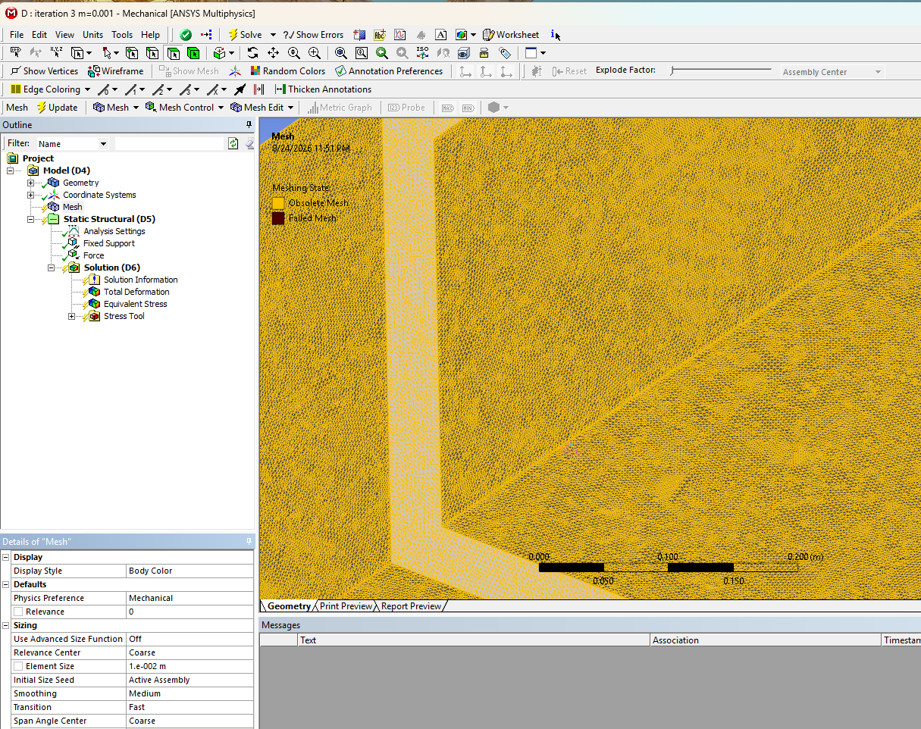
\includegraphics[width=0.48\textwidth]{mallado_003_punto1.png}
\caption{Detalle de malla -- barra de hormigón, Punto 1, \textit{sizing} de 0.03 m}
\label{fig:p1_mallado_003}
\end{figure}

\begin{figure}[H]
\centering
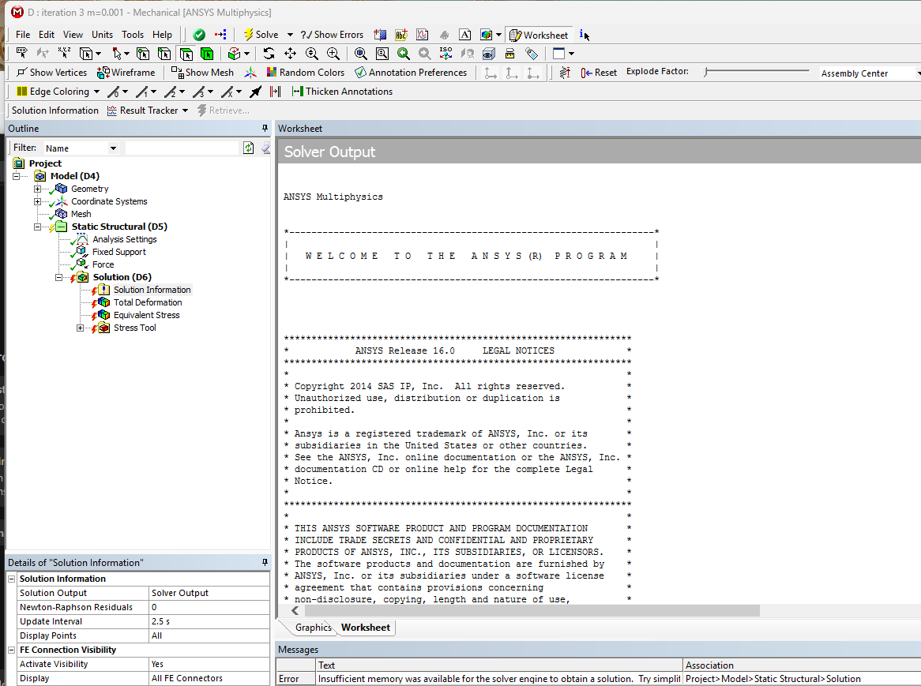
\includegraphics[width=0.48\textwidth]{error_malla_0005_punto1.png}
\caption{Error de solución -- intento de mallado con \textit{sizing} de 0.005 m: memoria insuficiente (\textit{``Insufficient memory was available for the solver engine''})}
\label{fig:p1_error_malla}
\end{figure}

Al intentar refinar la malla hasta un \textit{sizing} de 0.005 m, ANSYS reportó un error de memoria insuficiente en el motor de solución (Fig.~\ref{fig:p1_error_malla}), por lo que ese tamaño de elemento no pudo resolverse en el equipo disponible y queda excluido de la curva de independencia de malla; esto constituye una limitación práctica del estudio (no un artefacto físico) y debe reportarse como tal.

\textit{Nota sobre la curva de independencia de malla:} para completar la curva de límite de malla solicitada en este punto (deformación máxima vs. número de nodos/elementos) es necesario tabular, para cada tamaño de elemento intentado, el número de nodos, el número de elementos y la deformación máxima resultante, tal como se hizo para el Punto 2 (Tabla~\ref{tab:p2b2_malla}, Fig.~\ref{fig:p2_curva_malla_real}). Hasta el momento se cuenta con el caso de \textit{sizing} 0.03 m (Fig.~\ref{fig:p1_mallado_003}) y con el caso fallido de 0.005 m (Fig.~\ref{fig:p1_error_malla}); faltan los puntos intermedios (por ejemplo 1.0, 0.5 y 0.1 m) para construir la tabla y la gráfica completas.

\subsection{1C. Cálculo del \% de error}

Comparando el desplazamiento del nodo 4 obtenido mediante el método de la matriz de rigidez (3 elementos) contra la solución analítica exacta:

\[
\text{Error}(\%)=\frac{u_4-\delta}{\delta}
\]
\[
=\frac{3.746\times10^{-4}-3.79\times10^{-4}}{3.79\times10^{-4}}=-0.0107
\]

El desplazamiento calculado mediante el método de la matriz de rigidez (3 elementos) es un \textbf{1.07\% menor} que el valor exacto, lo cual confirma que una discretización relativamente gruesa (3 elementos) es suficiente para aproximar con buena precisión el comportamiento axial de esta barra.

Adicionalmente, comparando el resultado de la matriz de rigidez contra la deformación obtenida en la simulación de ANSYS (Fig.~\ref{fig:p1_deformacion}):
\[
\text{Error}(\%)=\frac{u_4-\delta_{ANSYS}}{\delta_{ANSYS}}
\]
\[
=\frac{3.746\times10^{-4}-3.8201\times10^{-4}}{3.8201\times10^{-4}}=-1.93\%
\]

Este valor deberá recalcularse una vez se cuente con la curva de independencia de malla completa (1B), tomando como referencia el valor de deformación correspondiente al mallado convergido (independiente de malla), y no únicamente el de una malla individual.

\section{Punto 2 -- Barra de hormigón de sección hueca}

En este segundo punto se analiza la misma barra de 2.80 m de longitud, ahora con una configuración de \textbf{sección hueca} de pared delgada, siguiendo el mismo procedimiento del punto anterior: discretización en tres elementos de sección uniforme, solución analítica por matriz de rigidez, simulación en ANSYS con su respectiva curva de independencia de malla, y cálculo del error entre ambos resultados.

\subsection{2A. Modelado por matriz de rigidez}

Se emplea la misma geometría externa del Punto 1 (base de 0.30 a 0.60 m, altura de 0.50 a 0.80 m, $L=2.80$ m), ahora con sección \textbf{hueca de pared delgada} y espesor constante $t=2$ mm, cargada axialmente con $P=15$ ton y módulo de elasticidad $E=2.1\times10^{7}$ ton/m$^2$ (valores propios del Punto 2).

\subsubsection*{Área neta de la sección hueca}

Las relaciones de la base y la altura externas en función de $z$ son las mismas del Punto 1:
\[
b_z(z)=0.1071\,z+0.3,\qquad h_z(z)=0.1071\,z+0.5
\]

Para una pared de espesor constante $t=0.002$ m, las dimensiones internas se reducen en $2t$ respecto a las externas ($b_i=b_z-2t$, $h_i=h_z-2t$), de modo que el área neta resulta:
\[
A_{neto}(z)=b_z h_z-b_i h_i = 2t\left[b_z(z)+h_z(z)\right]-4t^2
\]
\[
A_{neto}(z)=0.004\left[b_z(z)+h_z(z)\right]-0.000016
\]

\subsubsection*{Solución exacta (Ley de Hooke)}

\[
b_z(z)+h_z(z)=\frac{3}{14}z+0.8 \;\Rightarrow\; A_{neto}(z)=0.00085714\,z+0.003184
\]
\[
\delta=\frac{P}{E}\int_0^{L}\frac{dz}{A_{neto}(z)}=\frac{15}{2.1\times10^{7}}\int_0^{2.8}\frac{dz}{0.00085714z+0.003184}
\]
\[
\textbf{Solución exacta: } \delta = 4.681\times10^{-4}\text{ m}
\]

\subsubsection*{Discretización en tres elementos}

Empleando los mismos tres tramos y coordenadas $z$ del Punto 1 ($z_1=2.333$, $z_2=1.4$, $z_3=0.467$ m), las áreas netas resultantes son:
\[
A_1=0.005184\ \text{m}^2,\quad A_2=0.004384\ \text{m}^2,\quad A_3=0.003584\ \text{m}^2
\]

\subsubsection*{Rigidez de los elementos}

\[
[k^1]=\begin{pmatrix}116640&-116640\\-116640&116640\end{pmatrix}
\]
\[
[k^2]=\begin{pmatrix}98640&-98640\\-98640&98640\end{pmatrix}
\]
\[
[k^3]=\begin{pmatrix}80640&-80640\\-80640&80640\end{pmatrix}
\]

Matriz de rigidez global (ensamblada):
\[
{\small
\mathbf{K}=
\begin{pmatrix}
116640 & -116640 & 0 & 0\\
-116640 & 215280 & -98640 & 0\\
0 & -98640 & 179280 & -80640\\
0 & 0 & -80640 & 80640
\end{pmatrix}}
\]

\subsubsection*{Vector de cargas y desplazamientos}

\[
\mathbf{F}=\begin{pmatrix}-15\\0\\0\\15\end{pmatrix}\text{ton},\qquad
\mathbf{a}=\begin{pmatrix}0\\u_2\\u_3\\u_4\end{pmatrix}
\]

\subsubsection*{Matriz reducida y cálculo de desplazamientos}

\[
\mathbf{K}_{red}=
\begin{pmatrix}
215280 & -98640 & 0\\
-98640 & 179280 & -80640\\
0 & -80640 & 80640
\end{pmatrix}
\]

\[
\begin{pmatrix}u_2\\u_3\\u_4\end{pmatrix}=\mathbf{K}_{red}^{-1}\begin{pmatrix}0\\0\\15\end{pmatrix}
\]

Por lo tanto, los desplazamientos nodales son:
\[
u_1=0,\quad u_2=1.286\times10^{-4}\text{ m}
\]
\[
u_3=2.807\times10^{-4}\text{ m},\quad u_4=4.667\times10^{-4}\text{ m}
\]

\subsection{2B. Simulación en ANSYS}

\textbf{Nota de corrección:} en una versión previa de esta sección se presentaba, como estudio de independencia de malla de la barra hueca, una tabla y una curva (836 a 26.111 nodos, deformación de 0,0040607 a 0,0041191 m) que originaban una discrepancia del $-88{,}6\,\%$ frente al modelo analítico de 2A, imposible de explicar tras verificar geometría y material. Se confirmó posteriormente que esas figuras corresponden en realidad a una corrida del \textbf{Punto 1} (barra maciza), no de la barra hueca del Punto 2, por lo que fueron \textbf{retiradas de esta sección}. El estudio de independencia de malla válido y verificado para la barra hueca (Punto 2) es el que se presenta a continuación.

Se realizó el estudio de independencia de malla para la barra hueca (barra dos, $P=15$ ton), empleando un modelo paramétrico en ANSYS Workbench con cuatro configuraciones de malla: un caso base (\texttt{A}, malla por defecto de ANSYS) y tres iteraciones de refinamiento uniforme (\texttt{B}, \texttt{C}, \texttt{D}), controladas mediante el parámetro de tamaño de elemento $m$ (Fig.~\ref{fig:p2_esquema_parametrico}).

\begin{figure}[H]
\centering
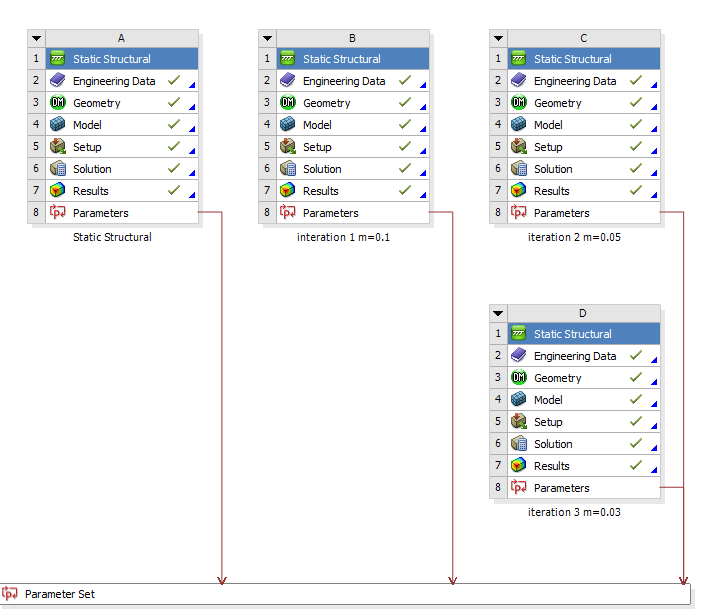
\includegraphics[width=0.48\textwidth]{esquema_parametrico_punto2b2.png}
\caption{Esquema paramétrico de las cuatro configuraciones de malla evaluadas -- Barra dos: caso base A y iteraciones B ($m=0.10$), C ($m=0.05$) y D ($m=0.03$)}
\label{fig:p2_esquema_parametrico}
\end{figure}

En los cuatro casos se aplicó la misma carga de $P=15$ ton ($1.471\times10^{5}$ N) sobre el extremo libre (Fig.~\ref{fig:p2b2_fuerza}), con la geometría y las condiciones de frontera de la barra hueca del Punto 2. Un quinto intento, con \textit{sizing} de 0.005 m, no pudo ejecutarse por falta de memoria de hardware disponible, de forma análoga a lo ocurrido en el Punto 1 (Fig.~\ref{fig:p1_error_malla}).

\begin{figure}[H]
\centering
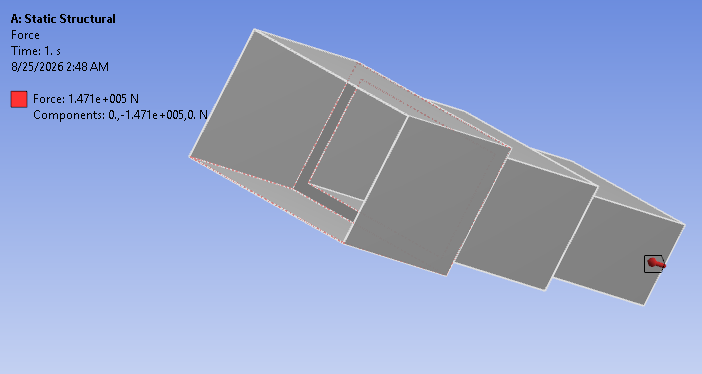
\includegraphics[width=0.45\textwidth]{fuerza_caso_a_punto2b2.png}
\caption{Carga aplicada -- $F=1.471\times10^{5}$ N ($P=15$ ton), caso base A}
\label{fig:p2b2_fuerza}
\end{figure}

\begin{table}[H]
\centering
\caption{Estudio paramétrico de malla A--D -- Barra dos (sección hueca)}
\label{tab:p2b2_malla}
\small
\begin{tabular}{@{}lcccc@{}}
\toprule
\textbf{Caso} & \textbf{Sizing (m)} & \textbf{Nodos} & \textbf{Elementos} & \textbf{Deform. máx. (m)} \\
\midrule
A & (por defecto) & 7\,603   & 3\,725  & $6.0828\times10^{-4}$ \\
B & 0.10          & 14\,300  & 7\,023  & $7.9601\times10^{-4}$ \\
C & 0.05          & 44\,307  & 21\,927 & $1.9131\times10^{-3}$ \\
D & 0.03          & 121\,331 & 60\,212 & $7.3496\times10^{-3}$ \\
E & 0.005         & \multicolumn{3}{c}{no convergió -- memoria insuficiente} \\
\bottomrule
\end{tabular}
\end{table}

\begin{figure}[H]
\centering
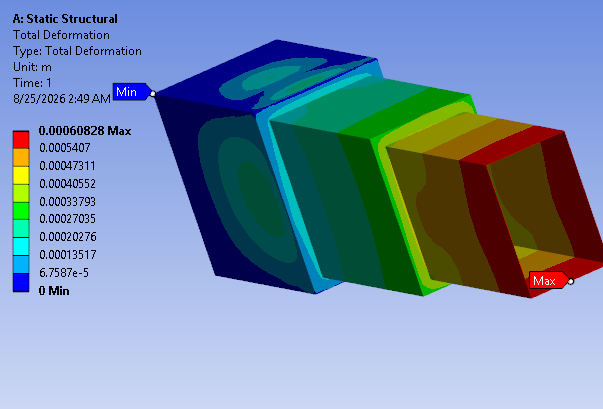
\includegraphics[width=0.44\textwidth]{deformacion_caso_a_punto2b2.png}
\caption{Deformación total -- caso A (malla por defecto), máx. $6.0828\times10^{-4}$ m}
\label{fig:p2b2_def_a}
\end{figure}

\begin{figure}[H]
\centering
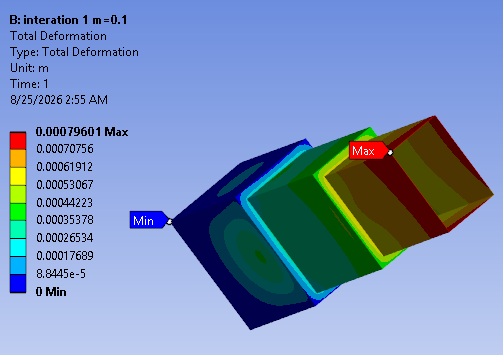
\includegraphics[width=0.44\textwidth]{deformacion_caso_b_punto2b2.png}
\caption{Deformación total -- caso B ($m=0.10$), máx. $7.9601\times10^{-4}$ m}
\label{fig:p2b2_def_b}
\end{figure}

\begin{figure}[H]
\centering
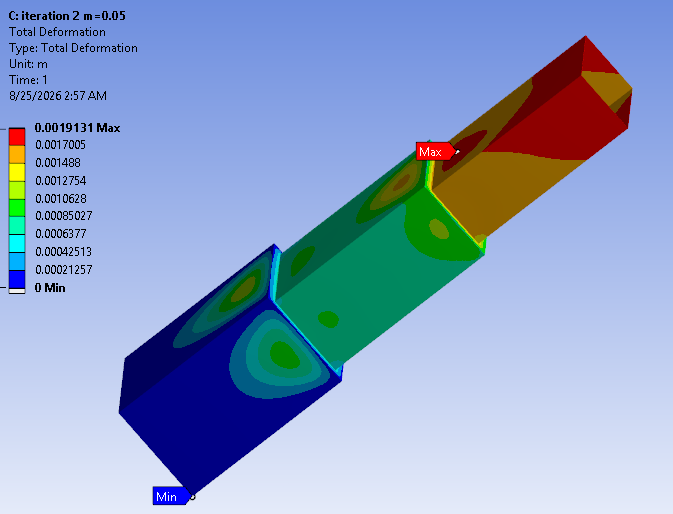
\includegraphics[width=0.44\textwidth]{deformacion_caso_c_punto2b2.png}
\caption{Deformación total -- caso C ($m=0.05$), máx. $1.9131\times10^{-3}$ m}
\label{fig:p2b2_def_c}
\end{figure}

\begin{figure}[H]
\centering
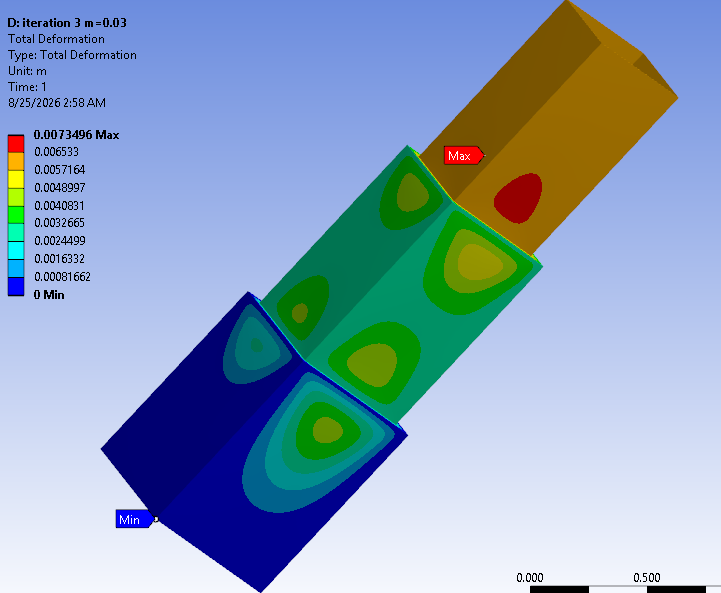
\includegraphics[width=0.44\textwidth]{deformacion_caso_d_punto2b2.png}
\caption{Deformación total -- caso D ($m=0.03$), máx. $7.3496\times10^{-3}$ m}
\label{fig:p2b2_def_d}
\end{figure}

\begin{figure}[H]
\centering
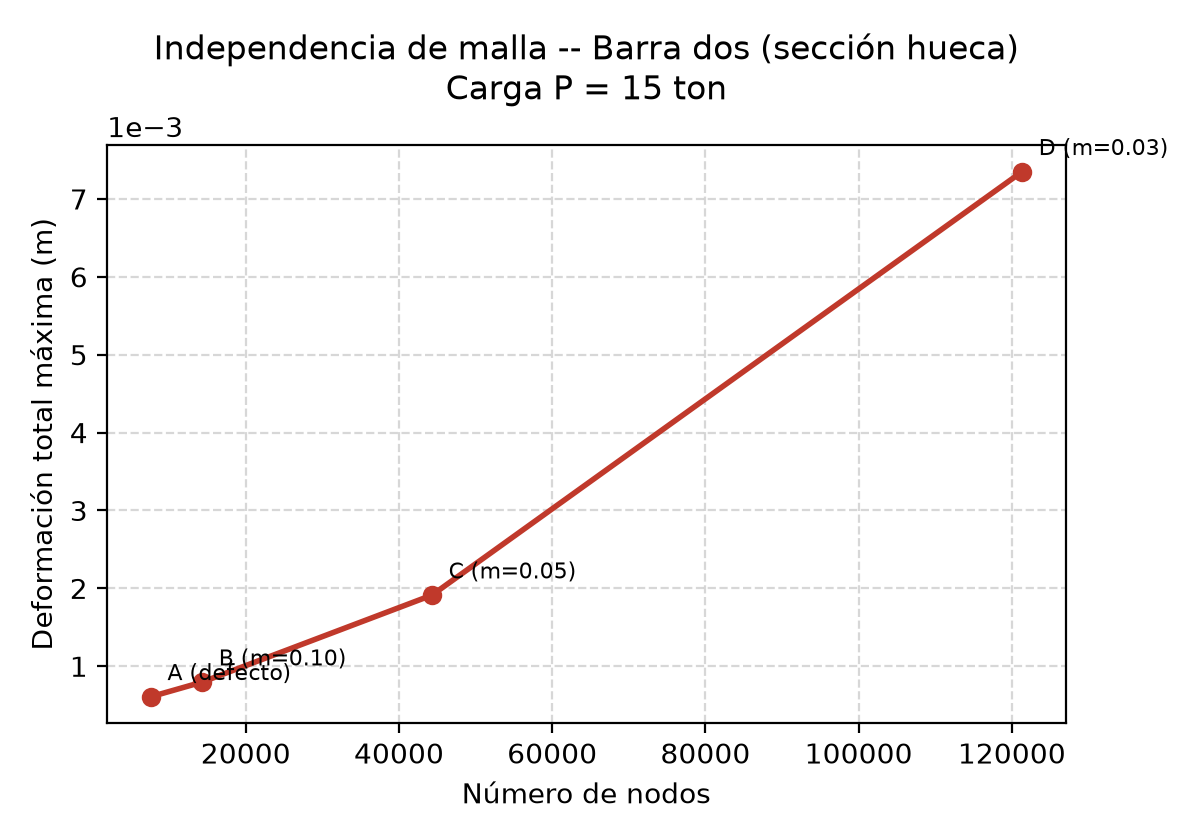
\includegraphics[width=0.48\textwidth]{malla_grafica_punto2b2.png}
\caption{Curva de independencia de malla -- Barra dos (sección hueca): número de nodos vs. deformación máxima, estudio paramétrico A--D}
\label{fig:p2_curva_malla_real}
\end{figure}

La curva (Fig.~\ref{fig:p2_curva_malla_real}) muestra que la deformación máxima \textbf{no converge}: crece de forma sostenida y acelerada con cada refinamiento (+30.9\,\% de A a B, +140.4\,\% de B a C, +284.3\,\% de C a D), sin ninguna zona de aplanamiento. Este comportamiento -- una magnitud que diverge en vez de estabilizarse a medida que la malla se refina -- es la firma característica de una \textbf{singularidad numérica}: un punto de aplicación de carga concentrada, una esquina reentrante en la transición entre los tres tramos de sección uniforme, o un apoyo idealizado como perfectamente rígido, todos ellos generan, en la teoría de elasticidad, esfuerzos y deformaciones que tienden matemáticamente a infinito en el punto singular; cuanto más fina es la malla, más se aproxima la solución numérica a ese valor no acotado, sin alcanzar nunca una independencia real de malla en esa zona.

Dado que este es el \textbf{único estudio de malla verificado para la barra hueca}, se adopta como \textbf{límite de malla} del Punto 2 el resultado del caso más refinado disponible, \texttt{D} ($m=0.03$, 121\,331 nodos, $\delta=7.3496\times10^{-3}$ m), ya que el intento de refinar más allá (sizing 0.005 m) no pudo ejecutarse por limitaciones de hardware. Se deja constancia de que la tendencia de la curva (Fig.~\ref{fig:p2_curva_malla_real}) aún no muestra una zona de aplanamiento -- a diferencia del Punto 1 -- por lo que este valor debe tratarse como la mejor estimación disponible con los recursos de cómputo actuales, y no como una independencia de malla estrictamente demostrada; de disponerse de mayor capacidad de cómputo, se recomienda extender el estudio con tamaños de malla más finos para confirmar si la curva efectivamente se estabiliza.

\begin{figure}[H]
\centering
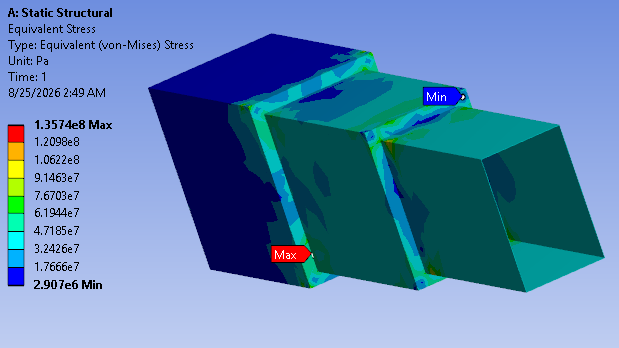
\includegraphics[width=0.44\textwidth]{esfuerzo_caso_a_punto2b2.png}
\caption{Esfuerzo equivalente (Von Mises) -- caso A: máx. $1.3574\times10^{8}$ Pa, mín. $2.907\times10^{6}$ Pa}
\label{fig:p2b2_esfuerzo_a}
\end{figure}

\begin{figure}[H]
\centering
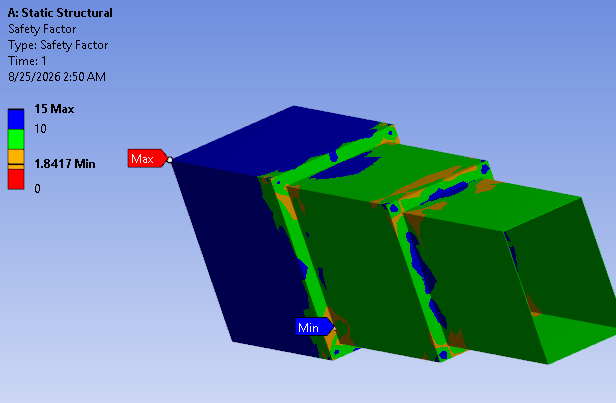
\includegraphics[width=0.42\textwidth]{factor_seguridad_caso_a_punto2b2.png}
\caption{Factor de seguridad -- caso A: máx. 15, mín. 1.8417}
\label{fig:p2b2_fs_a}
\end{figure}

El esfuerzo equivalente y el factor de seguridad del caso A (Figs.~\ref{fig:p2b2_esfuerzo_a}--\ref{fig:p2b2_fs_a}) también reflejan la concentración de esfuerzo en la zona de menor sección: el mínimo factor de seguridad (1.8417) se ubica en el extremo de sección más reducida, coherente con el mismo mecanismo de concentración de esfuerzo señalado para la deformación.

\subsection{2C. Cálculo del \% de error}

Comparando el desplazamiento del nodo 4 obtenido mediante el método de la matriz de rigidez (3 elementos) contra la solución analítica exacta (2A):
\[
\text{Error}(\%)=\frac{u_4-\delta}{\delta}=\frac{4.667\times10^{-4}-4.681\times10^{-4}}{4.681\times10^{-4}}=-0.31\%
\]

El desplazamiento calculado mediante el método de la matriz de rigidez (3 elementos) es un \textbf{0.31\% menor} que el valor exacto, un error del mismo orden de magnitud que el obtenido en el Punto 1 (-1.07\,\%), lo que confirma que la discretización en 3 elementos también es adecuada para la sección hueca.

\textbf{Comparación con la simulación en ANSYS:} la tabla y la curva que originalmente se presentaban en esta sección como el estudio de malla del Punto 2 ($\delta_{ANSYS}\approx4.1\times10^{-3}$ m) se identificaron como pertenecientes al Punto 1, no a la barra hueca (ver nota de corrección en 2B), por lo que ese valor se descarta. Tomando en su lugar el límite de malla adoptado en 2B para la barra hueca ($\delta_{ANSYS}=7.3496\times10^{-3}$ m, caso \texttt{D}, la malla más refinada disponible):
\[
\text{Error}(\%)=\frac{u_4-\delta_{ANSYS}}{\delta_{ANSYS}}=\frac{4.667\times10^{-4}-7.3496\times10^{-3}}{7.3496\times10^{-3}}\approx-93.65\%
\]

Este error es considerablemente mayor que el obtenido en el Punto 1 ($-1.93\,\%$). Se verificaron la geometría (SolidWorks: longitud de 2.80 m, dimensiones externas de los elementos 1 y 3, y espesor de pared de 2 mm, todas coincidentes con 2A) y el material ($E$ del acero estructural, cercano al valor de diseño), por lo que ninguna de las dos explica esta magnitud de error; sumado a que la curva de malla del Punto 2 aún no se aplana (2B), el error del $-93.65\,\%$ debe interpretarse como una cota superior provisional, condicionada a que el estudio de malla del Punto 2 todavía no alcanza una independencia de malla estrictamente demostrada.

\section{Punto 3 -- Viga de acero de perfil ``I'' (MATLAB PDE Tool)}

Este punto se aparta del modelo de barra unidimensional de los puntos anteriores para abordar un análisis de esfuerzo plano en dos dimensiones: se evalúan la deformación y los esfuerzos generados en un perfil de acero tipo ``I'' al aplicarle, sobre su cara superior, una carga total de 50 toneladas en dirección de compresión axial, con la base del perfil empotrada. El problema se resuelve mediante elementos finitos triangulares CST (\textit{Constant Strain Triangle}) programados manualmente, empleando la herramienta PDE Tool de MATLAB únicamente para la generación de la geometría y la malla.

\subsection{3A. Metodología}

Se empleó el método de los elementos finitos con elementos triangulares de deformación constante (CST) de 3 nodos, bajo la hipótesis de esfuerzo plano (\textit{plane stress}). El ensamblaje de la matriz de rigidez, la aplicación de las condiciones de frontera y la solución del sistema se programaron manualmente en MATLAB; la PDE Toolbox se utilizó únicamente para generar la geometría y la malla (funciones \texttt{decsg}, \texttt{initmesh} y \texttt{refinemesh}), sin emplear su solucionador interno. Este enfoque se basó en un código de referencia entregado por el docente para un ejercicio previo (una placa rectangular con un agujero circular sometida a tracción), adaptado para este caso a la geometría, las condiciones de frontera y la carga del perfil ``I''.

\subsection{3B. Geometría y propiedades del material}

El perfil se definió como un polígono de 12 vértices (coordenadas en mm, Tabla~\ref{tab:vertices_p3}): las alas superior e inferior tienen un ancho $B=700$ mm y un espesor $t_f=100$ mm cada una; el alma tiene un ancho $b_w=200$ mm (entre $x=250$ mm y $x=450$ mm) y la altura total del perfil es $H=380$ mm.

\begin{table}[H]
\centering
\caption{Vértices del polígono del perfil ``I'' (mm)}
\label{tab:vertices_p3}
\small
\begin{tabular}{@{}cc|cc@{}}
\toprule
\textbf{Vértice} & \textbf{(x,y)} & \textbf{Vértice} & \textbf{(x,y)} \\
\midrule
1 & (0,0)     & 7  & (700,380) \\
2 & (700,0)   & 8  & (0,380)   \\
3 & (700,100) & 9  & (0,280)   \\
4 & (450,100) & 10 & (250,280) \\
5 & (450,280) & 11 & (250,100) \\
6 & (700,280) & 12 & (0,100)   \\
\bottomrule
\end{tabular}
\end{table}

El perfil es de acero, con módulo de elasticidad $E=2\times10^{11}$ Pa (200\,000 MPa), coeficiente de Poisson $\nu=0.3$ y espesor fuera del plano $t=12$ mm. La matriz constitutiva de esfuerzo plano empleada es:
\[
D=\frac{E}{1-\nu^2}\begin{pmatrix}1 & \nu & 0\\ \nu & 1 & 0\\ 0 & 0 & \dfrac{1-\nu}{2}\end{pmatrix}
\]

\begin{figure}[H]
\centering
\includegraphics[width=0.48\textwidth]{malla_perfil_I_punto3.png}
\caption{Malla de elementos finitos triangulares sobre el perfil ``I'' (Punto 3)}
\label{fig:p3_malla}
\end{figure}

La malla (Fig.~\ref{fig:p3_malla}) muestra una discretización más densa en la zona del alma y en la transición ala-alma, donde se concentra la mayor complejidad geométrica y, según la teoría, la mayor concentración de esfuerzos.

\begin{figure}[H]
\centering
\includegraphics[width=0.48\textwidth]{numeros_elementos_punto3.png}
\caption{Numeración de los elementos triangulares del perfil ``I'' (Punto 3)}
\label{fig:p3_numeros}
\end{figure}

La Fig.~\ref{fig:p3_numeros} muestra la numeración interna asignada a cada elemento, empleada para la trazabilidad de los resultados de esfuerzo y deformación reportados en las secciones 3F y 3G.

\subsection{3C. Condiciones de frontera y carga}

Se restringieron completamente ($u_x=u_y=0$) todos los nodos ubicados en la base del perfil ($y=0$), simulando un empotramiento rígido, como el de una columna anclada a una base. El peso de 50 ton se convirtió a Newtons mediante $1\text{ ton-f}\approx9810$ N, obteniendo una carga total de $P=490\,500$ N, la cual se distribuyó uniformemente, en dirección vertical negativa, entre todos los nodos del borde superior ($y=380$ mm), representando una carga de compresión axial uniforme sobre la cara superior del perfil.

\subsection{3D. Formulación del elemento CST}

Para cada elemento triangular con nodos $(x_1,y_1)$, $(x_2,y_2)$, $(x_3,y_3)$ se definen las constantes geométricas:
\[
b_i=y_2-y_3,\quad b_j=y_3-y_1,\quad b_k=y_1-y_2
\]
\[
c_i=x_3-x_2,\quad c_j=x_1-x_3,\quad c_k=x_2-x_1
\]
\[
2A=x_1(y_2-y_3)+x_2(y_3-y_1)+x_3(y_1-y_2)
\]
con $A$ el área del triángulo. La matriz de deformación-desplazamiento es:
\[
B=\frac{1}{2A}\begin{pmatrix}b_i&0&b_j&0&b_k&0\\0&c_i&0&c_j&0&c_k\\c_i&b_i&c_j&b_j&c_k&b_k\end{pmatrix}
\]
y la matriz de rigidez del elemento:
\[
K^e = t\cdot A\cdot B^{T}\, D\, B
\]
Las matrices elementales (de $6\times6$, 2 grados de libertad por nodo) se ensamblan en la matriz de rigidez global $KK$, dando lugar al sistema
\[
KK\,U=F.
\]
Tras reducir el sistema eliminando los grados de libertad restringidos en la base, se resuelve
\[
U = KK_{red}^{-1}\,F_{red},
\]
y, para cada elemento, se recuperan las deformaciones y los esfuerzos mediante:
\[
\varepsilon = B\,U^e, \qquad \sigma = D\,\varepsilon.
\]

\subsection{3E. Proceso de desarrollo}

El desarrollo del modelo siguió un proceso iterativo de adaptación y depuración a partir del código de referencia entregado por el docente:

\begin{enumerate}
    \item Se adaptó la geometría del código de referencia (placa con agujero circular) a la del perfil ``I'', definiendo sus 12 vértices (Tabla~\ref{tab:vertices_p3}).
    \item En un primer intento se generó la geometría y la malla de forma interactiva con \textit{PDE Modeler} (\texttt{pdetool}), replicando el flujo de trabajo del ejemplo del docente. Al ejecutar el script completo se obtuvo el error \texttt{Unrecognized function or variable 'p'}, ya que la ventana interactiva de PDE Modeler no exporta automáticamente las matrices de malla (\texttt{p}, \texttt{e}, \texttt{t}) al \textit{workspace} de MATLAB; esto solo ocurre si se realiza manualmente mediante \textit{Mesh} $\rightarrow$ \textit{Export Mesh}.
    \item Se corrigió el enfoque generando la geometría y la malla de forma completamente programática, con las funciones \texttt{decsg} (matriz de descripción de geometría), \texttt{initmesh} (malla inicial) y \texttt{refinemesh} (refinamiento), que devuelven \texttt{p}, \texttt{e} y \texttt{t} directamente como salidas de función, sin depender de ninguna ventana interactiva.
    \item Como parte de la verificación de la geometría durante esta depuración, se resolvió también la ecuación escalar genérica de prueba del propio PDE Modeler sobre el perfil (Fig.~\ref{fig:p3_color_u}); este resultado \textbf{no corresponde al análisis estructural} desarrollado en el informe, sino que se incluye únicamente como evidencia del proceso de verificación de la geometría, previo al ensamblaje del modelo CST.
    \item Con la malla ya disponible en el formato correcto, se ejecutó el ensamblaje de la matriz de rigidez CST, se aplicaron las condiciones de frontera (empotramiento en la base, carga distribuida en el borde superior), se resolvió el sistema reducido y se calcularon los esfuerzos y las deformaciones por elemento.
    \item Finalmente, se generaron las visualizaciones de resultados coloreando el centroide de cada elemento según su valor normalizado de esfuerzo o deformación.
\end{enumerate}

\begin{figure}[H]
\centering
\includegraphics[width=0.48\textwidth]{color_u_debug_punto3.png}
\caption{Figura de depuración -- solución genérica de prueba en PDE Modeler sobre la geometría del perfil ``I'' (no corresponde al análisis estructural)}
\label{fig:p3_color_u}
\end{figure}

\subsection{3F. Resultados: esfuerzos}

\begin{figure}[H]
\centering
\includegraphics[width=0.48\textwidth]{esfuerzo_sx_punto3.png}
\caption{Esfuerzo normal $\sigma_x$ (normalizado) -- perfil ``I'' (Punto 3)}
\label{fig:p3_sx}
\end{figure}

La distribución del esfuerzo normal horizontal $\sigma_x$ (Fig.~\ref{fig:p3_sx}) se mantiene baja en la mayor parte del perfil, con valores más altos (normalizados por encima de 0.6) concentrados en algunos elementos aislados de las alas, cerca de su transición con el alma. Al no ser esta la dirección de la carga aplicada, su magnitud es en general menor que la del esfuerzo $\sigma_y$.

\begin{figure}[H]
\centering
\includegraphics[width=0.48\textwidth]{esfuerzo_sy_punto3.png}
\caption{Esfuerzo normal $\sigma_y$ (normalizado) -- perfil ``I'' (Punto 3)}
\label{fig:p3_sy}
\end{figure}

El esfuerzo normal vertical $\sigma_y$ (Fig.~\ref{fig:p3_sy}), en la dirección de la carga aplicada, es el esfuerzo dominante en este problema de compresión axial. Los valores máximos (normalizados, cercanos a 1) se concentran en las esquinas reentrantes de la transición ala-alma, mientras que en el alma -- de menor área transversal que las alas -- los valores son consistentemente más altos que en las alas, lo cual es coherente con la relación $\sigma=F/A$: a menor área, mayor esfuerzo para una misma carga.

\begin{figure}[H]
\centering
\includegraphics[width=0.48\textwidth]{esfuerzo_txy_punto3.png}
\caption{Esfuerzo cortante $\tau_{xy}$ (normalizado) -- perfil ``I'' (Punto 3)}
\label{fig:p3_txy}
\end{figure}

El esfuerzo cortante en el plano $\tau_{xy}$ (Fig.~\ref{fig:p3_txy}) se concentra principalmente en las esquinas reentrantes donde el alma se une con las alas, actuando estas como concentradores de esfuerzo geométricos, típicos de cambios abruptos de sección en el análisis por elementos finitos.

\subsection{3G. Resultados: deformaciones}

\begin{figure}[H]
\centering
\includegraphics[width=0.48\textwidth]{deformacion_ex_punto3.png}
\caption{Deformación $\varepsilon_x$ (normalizada) -- perfil ``I'' (Punto 3)}
\label{fig:p3_ex}
\end{figure}

\begin{figure}[H]
\centering
\includegraphics[width=0.48\textwidth]{deformacion_ey_punto3.png}
\caption{Deformación $\varepsilon_y$ (normalizada) -- perfil ``I'' (Punto 3)}
\label{fig:p3_ey}
\end{figure}

\begin{figure}[H]
\centering
\includegraphics[width=0.48\textwidth]{deformacion_gxy_punto3.png}
\caption{Deformación angular $\gamma_{xy}$ (normalizada) -- perfil ``I'' (Punto 3)}
\label{fig:p3_gxy}
\end{figure}

Los campos de deformación $\varepsilon_x$, $\varepsilon_y$ y $\gamma_{xy}$ (Figs.~\ref{fig:p3_ex}--\ref{fig:p3_gxy}) siguen el mismo patrón espacial que sus respectivos esfuerzos, como es de esperarse de la relación constitutiva $\sigma=D\varepsilon$: las mayores deformaciones normales en $y$ se concentran en el alma y en las esquinas reentrantes, y las mayores deformaciones angulares coinciden con las zonas de mayor esfuerzo cortante.

\subsection{3H. Discusión}

Los resultados obtenidos son consistentes con el comportamiento esperado de un perfil ``I'' bajo compresión axial: el alma, al tener una sección transversal considerablemente menor que las alas, concentra los mayores esfuerzos normales $\sigma_y$; las esquinas reentrantes de la transición ala-alma, por su cambio abrupto de geometría, actúan como concentradores tanto de esfuerzo cortante $\tau_{xy}$ como, en menor medida, de esfuerzo normal $\sigma_x$.

Cabe señalar que todos los valores mostrados en las figuras están normalizados (escala de 0 a 1) respecto al valor absoluto máximo de cada variable; para obtener los valores físicos reales en MPa, estos deben extraerse directamente de las variables \texttt{ESFUERZOTOTAL} y \texttt{DEFORMACIONTOTAL} del \textit{workspace} de MATLAB antes de la normalización.

\section{Punto 4 -- Simulación térmica de un caldo de costilla en olla de aluminio (ANSYS 3D)}

Este punto traslada el análisis por elementos finitos a un problema de transferencia de calor en régimen estacionario, aplicado a un caso cotidiano: un caldo de costilla con dos papas dispuesto al interior de una olla de aluminio de 5 litros. El problema se resuelve mediante un modelo térmico tridimensional en el módulo \textit{Steady-State Thermal} de ANSYS, evaluando la distribución de temperatura y el flujo de calor resultantes de las propiedades térmicas de los materiales involucrados y de las condiciones de frontera impuestas sobre el sistema.

\subsection{4A. Configuración del modelo}

La olla se modeló en aluminio, material de alta conductividad térmica ($k\approx205$ W/m$\cdot$K), lo que favorece una distribución de temperatura relativamente uniforme en las paredes del recipiente. En su interior se incluyó un cuerpo de agua que representa el caldo, el cual se ocultó (\textit{hide}) en las vistas para poder visualizar la costilla y las dos papas dispuestas dentro de la olla. A la costilla y a las papas se les asignaron las propiedades térmicas del material carbono como aproximación, dado que ANSYS no cuenta en su librería estándar con propiedades térmicas específicas para alimentos como la papa o la carne; el carbono se utilizó como material sustituto para poder ejecutar la simulación conservando un sólido con conductividad térmica definida en el interior del caldo.

\subsection{4B. Resultados de la simulación}

\begin{figure}[H]
\centering
\includegraphics[width=0.48\textwidth]{temperatura_punto4.png}
\caption{Distribución de temperatura -- olla de aluminio con caldo de costilla (Punto 4)}
\label{fig:p4_temperatura}
\end{figure}

La distribución de temperatura (Fig.~\ref{fig:p4_temperatura}) muestra un núcleo interior -- caldo, papas y costilla -- prácticamente uniforme y cercano al valor máximo de $\mathbf{203.97\,^{\circ}\text{C}}$, mientras que la pared de aluminio presenta un gradiente que decrece desde la base (zona de mayor temperatura, en contacto con la fuente de calor) hacia el borde superior y las asas, donde se registran los valores mínimos, de hasta $92\,^{\circ}$C. Este comportamiento es coherente con la alta conductividad térmica del aluminio, que conduce el calor eficientemente a lo largo de las paredes de la olla, mientras que las asas, al estar más alejadas de la fuente de calor y más expuestas al ambiente, actúan como zonas de disipación y presentan las temperaturas más bajas del modelo.

\begin{figure}[H]
\centering
\includegraphics[width=0.48\textwidth]{flujo_calor_total_punto4.png}
\caption{Flujo de calor total -- olla de aluminio con caldo de costilla (Punto 4)}
\label{fig:p4_flujo_total}
\end{figure}

El flujo de calor total (Fig.~\ref{fig:p4_flujo_total}) alcanza un valor máximo de $5.5656\times10^{5}$ W/m$^2$, concentrado principalmente en la interfaz entre el contenido sólido interior (costilla y papas, modeladas con carbono) y el caldo, donde el gradiente térmico es más pronunciado debido a la diferencia de propiedades térmicas entre los materiales. En la pared de aluminio el flujo se distribuye de forma más homogénea, lo cual es consistente con su alta conductividad térmica: el calor se conduce eficientemente a través del metal sin generar concentraciones tan marcadas como las observadas en las interfaces internas del alimento.

\begin{figure}[H]
\centering
\includegraphics[width=0.48\textwidth]{flujo_calor_direccional_punto4.png}
\caption{Flujo de calor direccional (eje X) -- olla de aluminio con caldo de costilla (Punto 4)}
\label{fig:p4_flujo_x}
\end{figure}

El flujo de calor direccional en el eje X (Fig.~\ref{fig:p4_flujo_x}) presenta valores que oscilan entre $-2.9629\times10^{5}$ y $2.8489\times10^{5}$ W/m$^2$, con la mayor parte del modelo en tonos verdes, es decir, con una componente de flujo en la dirección X cercana a cero. Esto indica que el flujo de calor dominante no ocurre preferencialmente sobre el eje X, sino que se distribuye de forma más simétrica en las direcciones radial y vertical, coherente con una fuente de calor ubicada en la base de la olla. Las zonas de mayor magnitud, visibles en tonos amarillo/naranja sobre el borde superior cerca de una de las asas, reflejan asimetrías locales de la geometría (la presencia de las asas) que generan componentes de flujo más marcadas en esa dirección particular.

\textit{Nota:} para completar el Punto 4 sería útil incorporar, si se dispone de ellas, las figuras del flujo de calor direccional en los ejes Y y Z, así como un mapa de las propiedades/materiales asignados en el modelo (aluminio, agua, carbono), para respaldar visualmente la configuración descrita en 4A.

\section{Punto 5 -- Simulación magnetostática de bobinas de Helmholtz (ANSYS 3D)}

Este punto amplía el alcance del MEF hacia el dominio electromagnético, mediante la simulación magnetostática tridimensional de un par de bobinas de Helmholtz utilizadas para la estimulación muscular del antebrazo, con el fin de caracterizar el campo magnético generado por la configuración de bobinas.

\subsection{5A. Metodología}

El problema se resolvió en el módulo \textit{Magnetostatic} de ANSYS, siguiendo el flujo de trabajo estándar de \textit{Engineering Data} $\rightarrow$ \textit{Geometry} $\rightarrow$ \textit{Model} $\rightarrow$ \textit{Setup} $\rightarrow$ \textit{Solution} $\rightarrow$ \textit{Results} (Fig.~\ref{fig:p5_workflow}), resolviendo las ecuaciones de Maxwell en su forma estacionaria (magnetostática) descritas en el Marco Teórico.

\begin{figure}[H]
\centering
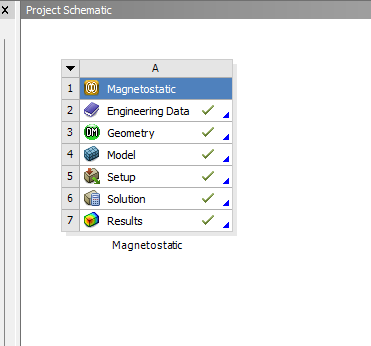
\includegraphics[width=0.45\textwidth]{esquema_workflow_punto5.png}
\caption{Esquema del proyecto (\textit{Project Schematic}) -- análisis Magnetostatic en ANSYS (Punto 5)}
\label{fig:p5_workflow}
\end{figure}

\subsection{5B. Geometría, materiales y condiciones de frontera}

El modelo está compuesto por cuatro partes (Fig.~\ref{fig:p5_arbol}): un dominio de aire (\texttt{air}) que envuelve el sistema, dos bobinas idénticas (\texttt{coil1}, \texttt{coil2}) y el antebrazo (\texttt{muscle}), ubicado entre ambas bobinas como región de interés para la estimulación.

\begin{itemize}
    \item \textbf{Diámetro de cada bobina:} 70 mm (radio $R=35$ mm).
    \item \textbf{Número de vueltas por bobina:} 15.
    \item \textbf{Corriente aplicada:} 100 A en cada bobina, mediante dos fuentes independientes (\texttt{Source Conductor}, \texttt{Source Conductor 2}), cada una con su condición \texttt{Current}.
    \item \textbf{Separación entre bobinas:} 70 mm (igual al diámetro, es decir, el doble del radio $R$).
    \item \textbf{Material de las bobinas:} \texttt{Copper Alloy} (propiedades por defecto de la librería de ANSYS).
    \item \textbf{Material del antebrazo (\texttt{muscle}):} material definido por el usuario, con permeabilidad relativa isotrópica $\mu_r=1$ y resistividad isotrópica $\rho=2\ \Omega\cdot$m.
    \item \textbf{Dominio circundante:} \texttt{Air}, con la condición de frontera \texttt{Magnetic Flux Parallel} aplicada en el límite exterior del dominio de aire (flujo magnético paralelo a la frontera, equivalente a una frontera de campo distante).
\end{itemize}

\begin{figure}[H]
\centering
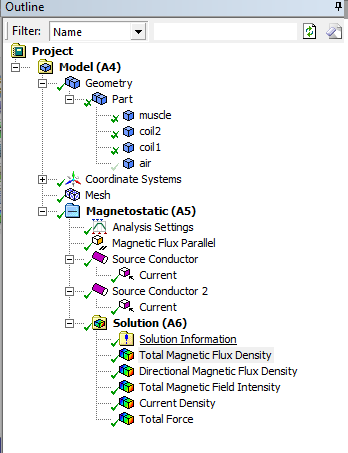
\includegraphics[width=0.4\textwidth]{arbol_geometria_bc_punto5.png}
\caption{Árbol del modelo -- geometría (\texttt{muscle}, \texttt{coil1}, \texttt{coil2}, \texttt{air}), condición \texttt{Magnetic Flux Parallel} y fuentes de corriente (Punto 5)}
\label{fig:p5_arbol}
\end{figure}

Cabe señalar que, para una configuración ideal de bobinas de Helmholtz, la separación entre bobinas debe ser igual al radio ($d=R=35$ mm); en este modelo la separación aplicada (70 mm) equivale al diámetro, es decir, el doble de la separación ideal. Esta desviación respecto a la condición de Helmholtz estricta se retoma en la discusión (5D).

\subsection{5C. Resultados}

\begin{figure}[H]
\centering
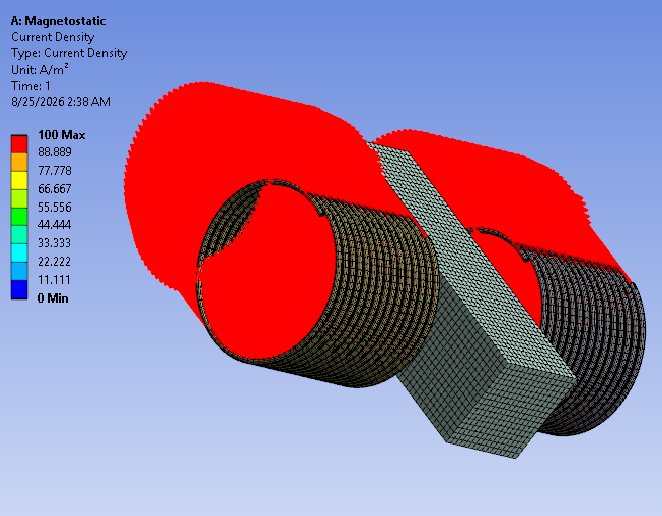
\includegraphics[width=0.48\textwidth]{densidad_corriente_punto5.png}
\caption{Densidad de corriente en las bobinas -- máximo 100 A/m$^2$ (Punto 5)}
\label{fig:p5_corriente}
\end{figure}

La Fig.~\ref{fig:p5_corriente} muestra la densidad de corriente resultante en el devanado de ambas bobinas, con un valor máximo de 100 A/m$^2$, correspondiente a la excitación de 100 A por bobina definida en la configuración del modelo.

\begin{figure}[H]
\centering
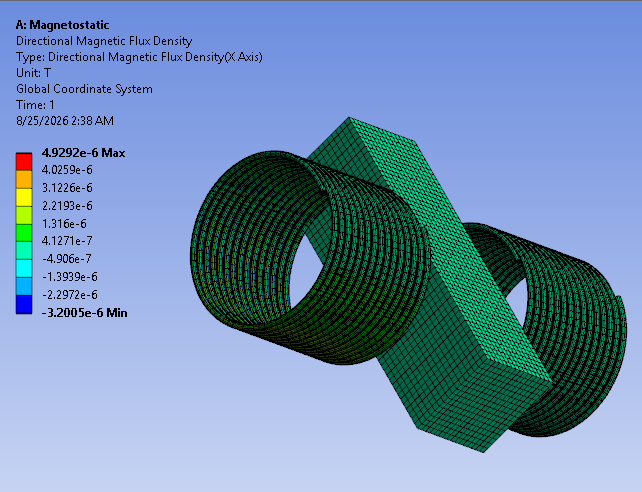
\includegraphics[width=0.48\textwidth]{flujo_direccional_x_punto5.png}
\caption{Densidad de flujo magnético direccional (eje X) -- máximo $4.9292\times10^{-6}$ T, mínimo $-3.2005\times10^{-6}$ T (Punto 5)}
\label{fig:p5_flujo_x}
\end{figure}

La densidad de flujo magnético direccional en el eje X (Fig.~\ref{fig:p5_flujo_x}) alcanza un valor máximo de $4.9292\times10^{-6}$ T y un mínimo de $-3.2005\times10^{-6}$ T, con el cambio de signo asociado al sentido del campo generado por cada bobina a ambos lados del eje común.

\begin{figure}[H]
\centering
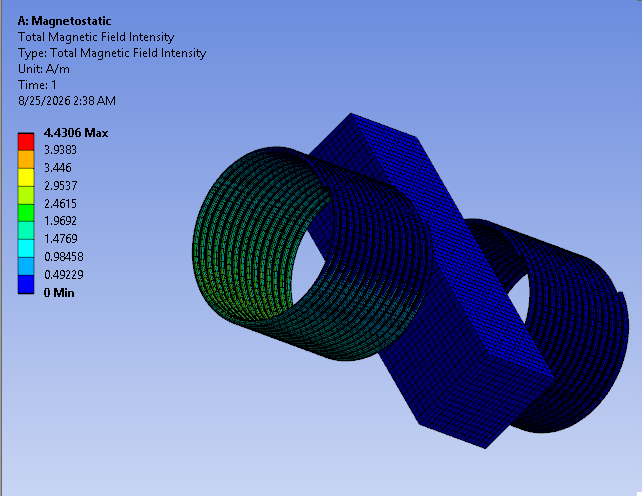
\includegraphics[width=0.48\textwidth]{intensidad_campo_punto5.png}
\caption{Intensidad de campo magnético total -- máximo 4.4306 A/m, mínimo 0 A/m (Punto 5)}
\label{fig:p5_intensidad}
\end{figure}

La intensidad de campo magnético total (Fig.~\ref{fig:p5_intensidad}) presenta su valor máximo de 4.4306 A/m en el interior de las bobinas, decreciendo hacia las regiones más alejadas del eje de simetría, donde se aproxima a cero.

\begin{figure}[H]
\centering
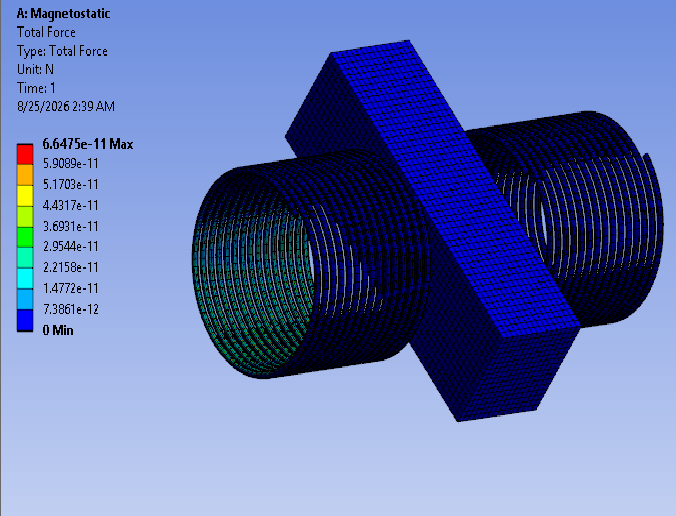
\includegraphics[width=0.48\textwidth]{fuerza_total_punto5.png}
\caption{Fuerza total sobre el sistema -- máximo $6.6475\times10^{-11}$ N, mínimo 0 N (Punto 5)}
\label{fig:p5_fuerza}
\end{figure}

La fuerza total calculada por ANSYS (Fig.~\ref{fig:p5_fuerza}) es del orden de $10^{-11}$ N, es decir, prácticamente despreciable, lo cual es coherente con una configuración de bobinas coaxiales y simétricas, donde las fuerzas de atracción/repulsión mutua tienden a cancelarse en la dirección axial.

\subsection{5D. Discusión y validación}

Como verificación de orden de magnitud, el campo magnético teórico en el punto medio de un par de bobinas de Helmholtz \emph{ideal} (separación $d=R$) está dado por
\[
B_{centro} = \left(\frac{4}{5}\right)^{3/2}\frac{\mu_0 N I}{R},
\]
con $\mu_0=4\pi\times10^{-7}$ H/m. Sustituyendo $N=15$, $I=100$ A y $R=0.035$ m se obtiene $B_{centro}\approx 38.5$ mT, varios órdenes de magnitud por encima de la densidad de flujo reportada por ANSYS ($\sim\!5\times10^{-6}$ T $=0.005$ mT). Esta discrepancia no debe interpretarse como una validación satisfactoria del modelo; por el contrario, señala una inconsistencia que debe revisarse antes de usar estos resultados para conclusiones cuantitativas sobre la intensidad de estimulación: entre las causas más probables están (i) que la separación real (70 mm, el doble del valor ideal $R$) reduce el campo respecto al caso ideal pero no explica por sí sola una diferencia de varios órdenes de magnitud, y (ii) que la excitación efectivamente resuelta por el solver ($100$ A/m$^2$ de densidad de corriente, Fig.~\ref{fig:p5_corriente}) podría no corresponder a los $100$ A concentrados en $15$ vueltas por bobina definidos como dato de entrada, sino a una densidad de corriente uniforme mucho menor en términos de amperios-vuelta efectivos. Se recomienda revisar en ANSYS la definición de la fuente de corriente (\texttt{Source Conductor}) para confirmar que el número de vueltas y la corriente por vuelta se hayan introducido correctamente antes de reportar estos valores como definitivos.

Adicionalmente, la separación entre bobinas empleada (70 mm) no corresponde a la condición de Helmholtz estricta ($d=R=35$ mm), sino al doble de esta, lo que en un caso ideal produciría un campo menos uniforme en la región central que el de una configuración de Helmholtz propiamente dicha; esto es relevante para la aplicación de estimulación muscular, donde la uniformidad del campo en la región del antebrazo es un criterio de diseño relevante.

\section{Conclusiones}
\begin{enumerate}
    \item El método de la matriz de rigidez con solo tres elementos de sección uniforme resultó suficientemente preciso frente a la solución analítica exacta tanto para la barra maciza (Punto 1, error de $-1.07\,\%$) como para la barra hueca (Punto 2, error de $-0.31\,\%$), confirmando que, para elementos axiales con variación suave de sección, una discretización gruesa ya captura el comportamiento global de la estructura. La comparación contra ANSYS, en cambio, dejó resultados muy distintos entre ambos puntos: en el Punto 1 el error frente a la simulación fue de apenas $-1.93\,\%$, mientras que en el Punto 2 el error frente al límite de malla adoptado fue de $-93.65\,\%$, explicado por que el estudio de malla propio de la barra hueca aún no muestra una zona de convergencia clara (la deformación sigue creciendo con el refinamiento, indicio de una posible singularidad numérica en el modelo de ANSYS). Esto evidencia la importancia de verificar el origen y la convergencia de cada resultado de simulación antes de usarlo como referencia de validación, en vez de asumir que cualquier salida de ANSYS es automáticamente correcta.

    \item El análisis del perfil ``I'' de acero (Punto 3) mediante elementos triangulares CST confirmó el comportamiento esperado de una sección con alma más delgada que las alas bajo compresión axial: el esfuerzo normal $\sigma_y$ domina sobre $\sigma_x$, se concentra principalmente en el alma (de menor área transversal) y en las esquinas reentrantes de la transición ala-alma, donde también se concentra el esfuerzo cortante $\tau_{xy}$; estas esquinas actúan como concentradores geométricos de esfuerzo, un efecto típico de cambios abruptos de sección que debe considerarse en el diseño de perfiles estructurales similares.

    \item La simulación térmica estacionaria de la olla con caldo de costilla (Punto 4) mostró que la alta conductividad térmica del aluminio ($k\approx205$ W/m$\cdot$K) homogeniza rápidamente la temperatura a lo largo de las paredes del recipiente, generando un gradiente decreciente desde la base (en contacto con la fuente de calor, hasta $203.97\,^{\circ}$C) hacia las asas (mínimo de $92\,^{\circ}$C), las cuales actúan como zonas de disipación por su mayor exposición al ambiente; esto confirma que, en utensilios metálicos de cocina, la geometría de las asas es un factor determinante en la distribución de temperatura superficial y en el riesgo de contacto térmico.

    \item La simulación magnetostática de las bobinas de Helmholtz (Punto 5) permitió obtener los campos de densidad de flujo magnético, intensidad de campo e interacción de fuerza entre bobinas, pero reveló una discrepancia de varios órdenes de magnitud entre el campo central estimado analíticamente ($\approx38.5$ mT, para $N=15$, $I=100$ A y $R=35$ mm) y el reportado por ANSYS ($\approx5\times10^{-6}$ T); dado que la separación real entre bobinas (70 mm, el doble del radio) tampoco corresponde a la condición ideal de Helmholtz ($d=R$), este punto queda como el de menor validación numérica del informe y requiere revisar la definición de la fuente de corriente en ANSYS antes de emplear estos resultados para conclusiones cuantitativas sobre la intensidad de estimulación muscular.
\end{enumerate}

\begin{thebibliography}{9}

\bibitem{zienkiewicz2013}
O. C. Zienkiewicz y R. L. Taylor,
\textit{The Finite Element Method}, 7th ed.
Butterworth-Heinemann, 2013.

\bibitem{bathe1996}
K. J. Bathe,
\textit{Finite Element Procedures}.
Prentice Hall, 1996.

\bibitem{logan2012}
D. L. Logan,
\textit{A First Course in the Finite Element Method}.
Cengage Learning, USA, 2012.

\bibitem{reddy2005}
J. N. Reddy,
\textit{An Introduction to the Finite Element Method}, 3rd ed.
McGraw-Hill, 2005.

\bibitem{incropera2011}
F. P. Incropera, D. P. DeWitt, T. L. Bergman y A. S. Lavine,
\textit{Fundamentals of Heat and Mass Transfer}, 7th ed.
John Wiley \& Sons, 2011.

\bibitem{sadiku2018}
M. N. O. Sadiku,
\textit{Elements of Electromagnetics}, 7th ed.
Oxford University Press, 2018.

\end{thebibliography}

\end{document}